\section{Introduction}



\section{Literature Review?}

\textcolor{red}{What are some of the novelties of this study}
\begin{enumerate}
    \item Multiple case study that looks at multiple scales of energy governance in the state of Illinois.
    Other studies that investigated multiple cases only looked at the energy policy and decision making at
    the municipal level \cite{johannsen_designing_2021, ben_amer_too_2020}.
    \item Considers structural barriers to energy modeling.
    \item Investigates the role concepts of energy justice do (or do not) play in energy policy for some 
    places in Illinois.
    \item Evaluates a specific energy modeling tool and features of that tool.
\end{enumerate}

\section{Methodology}

\subsection{Thematic Analysis}
This thesis relies on multiple case studies using interviews with energy planners and decision makers at local
and state levels, extending the method described by Johannsen et al. 2021 \cite{johannsen_designing_2021}. The
interviewees were chosen to be paradigmatic cases (\textcolor{red}{Is this really what I mean?}) \cite{flyvbjerg_five_2006}.
The interviews were transcribed with the ``listen and revise method'' using the Whisper transcription tool \cite{battaglia_listen_2024}. Whisper uses \ac{ai} to automate the transcription
process. Both the data and the \ac{ai} model used to transcribe the interview audio were hosted locally (i.e., without an internet
connection), eliminating privacy concerns \cite{battaglia_listen_2024}. Figure \ref{fig:whisper} shows a screenshot of the 
Whisper interface. The interview coding step was also performed locally with
the \texttt{Taguette} tool \cite{rampin_taguette_2021}. Figure \ref{fig:taguette} shows a screenshot of the \texttt{Taguette}
software.

\begin{figure}
    \centering
    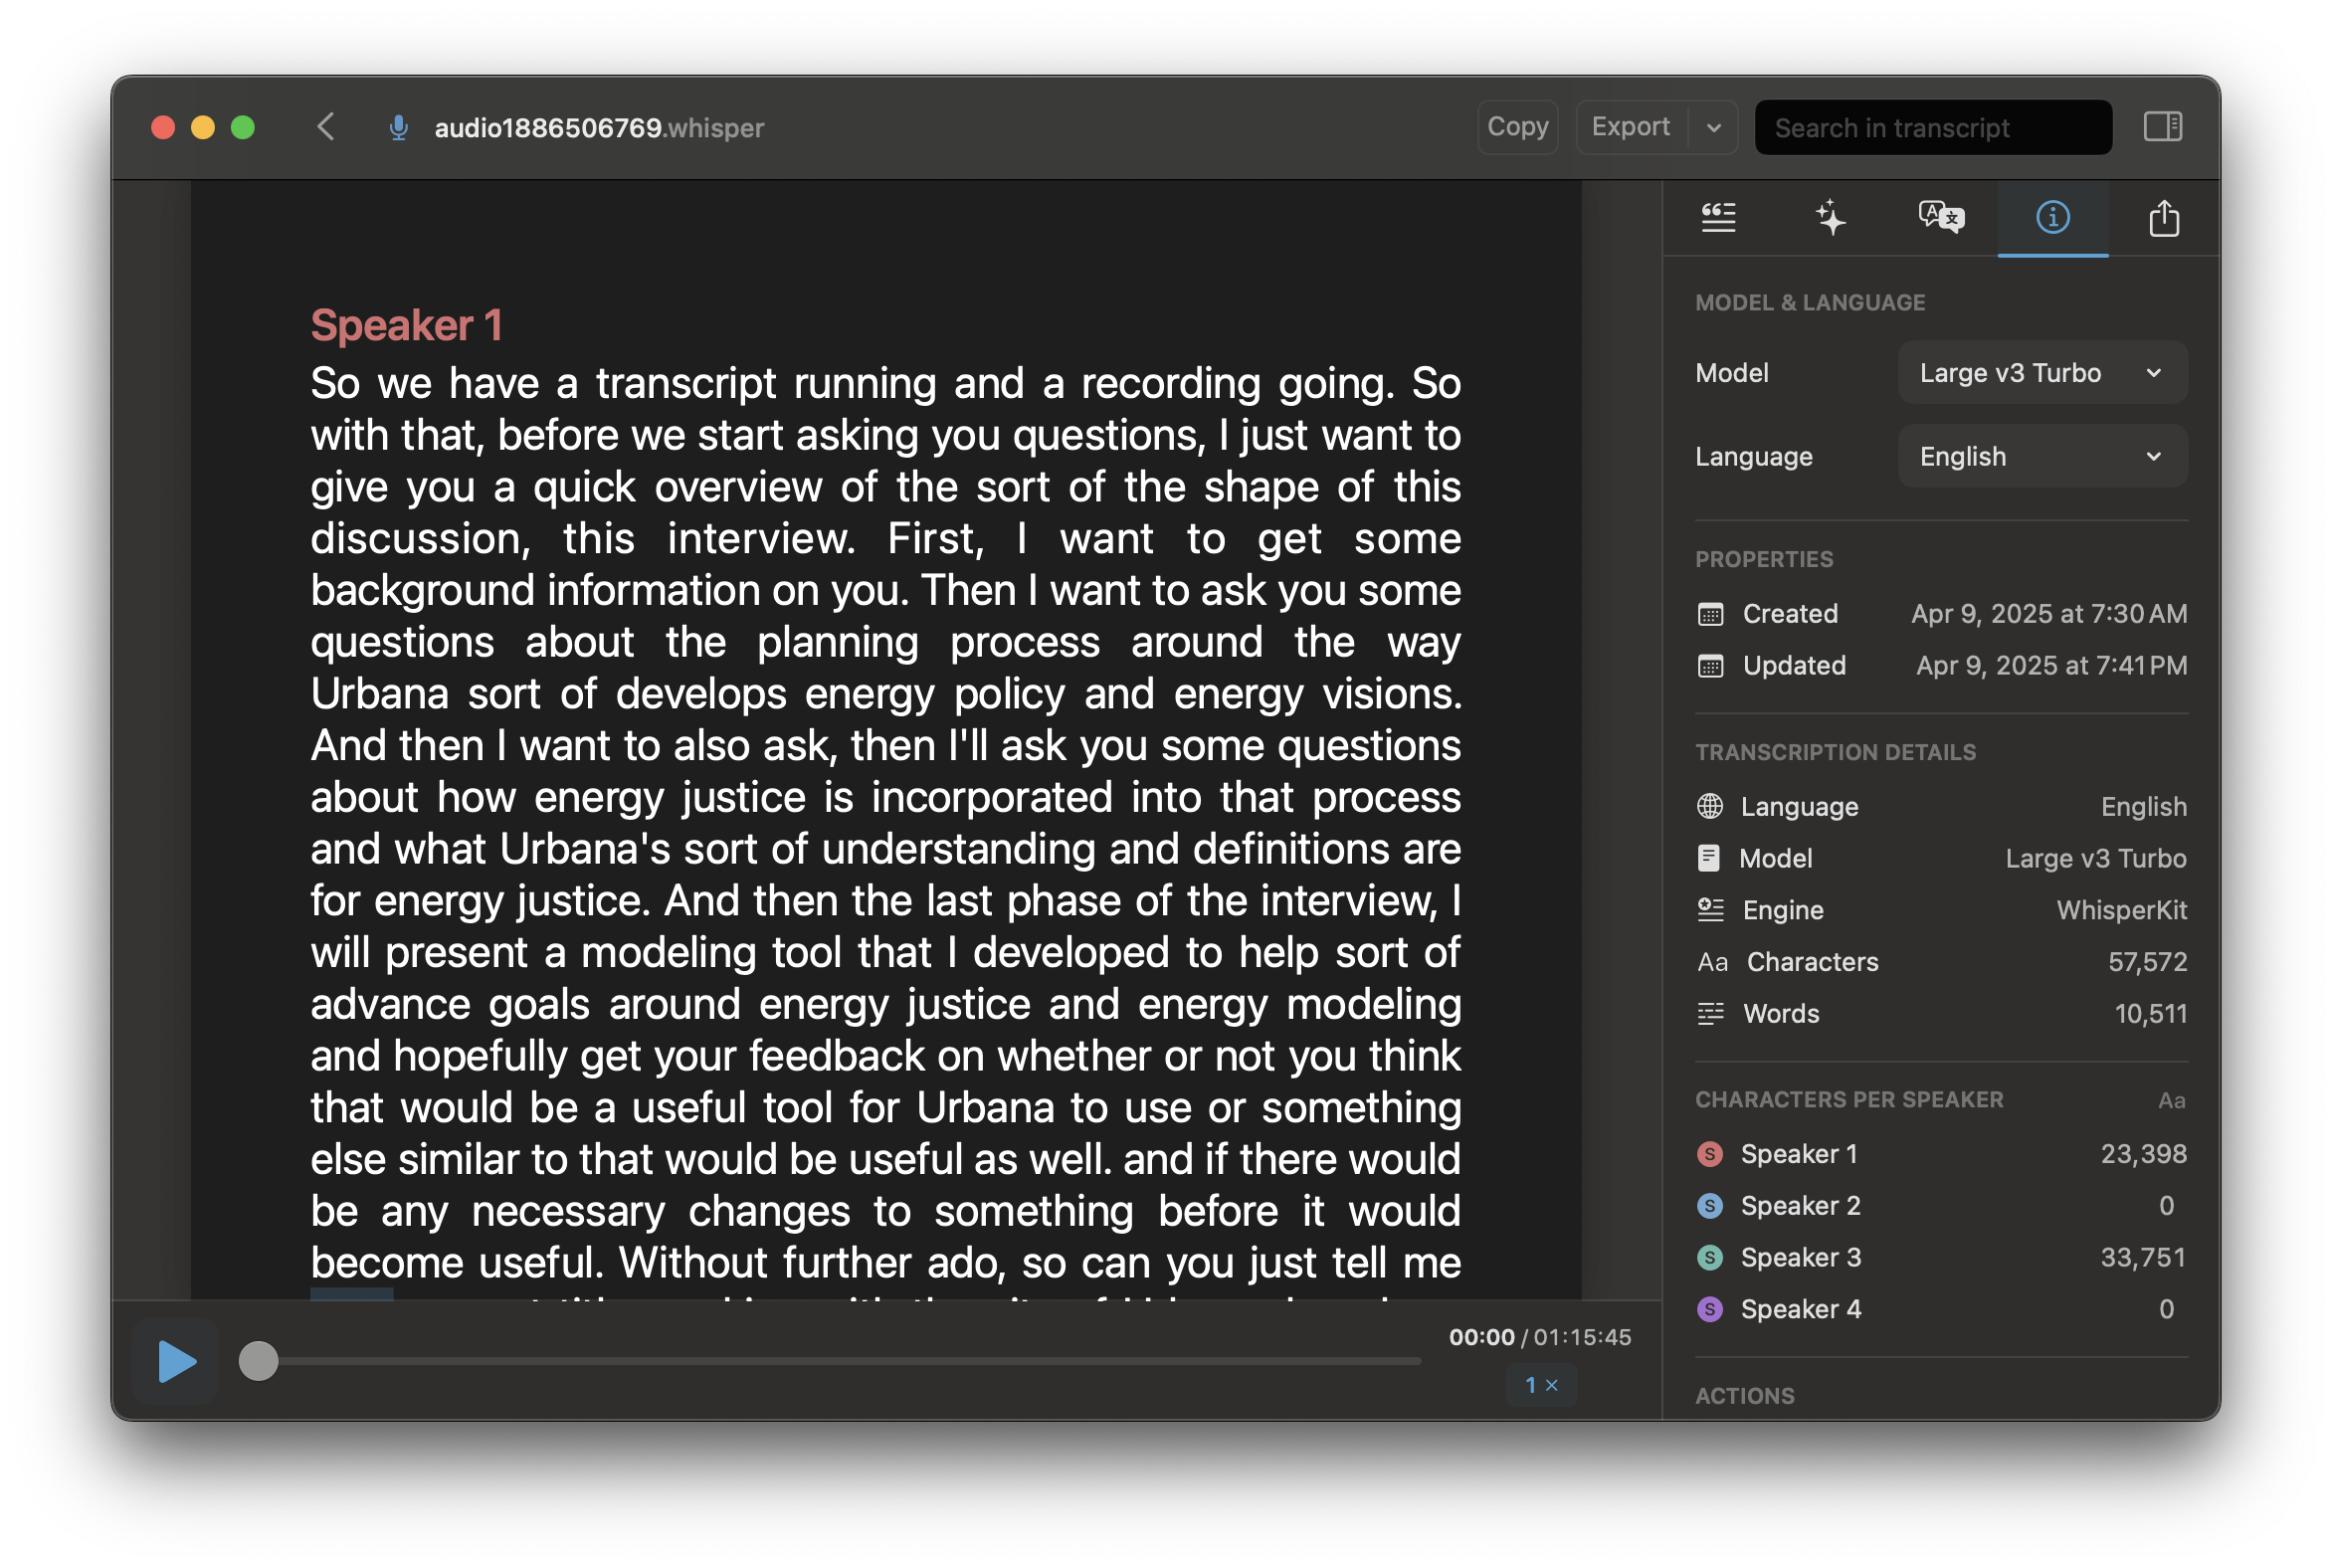
\includegraphics[width=0.6\columnwidth]{figures/07_interview_chapter/whisper-screenshot.png}
    \caption{A screenshot of an interview transcribed with Whisper. To protect the privacy of the interviewees, only ``Speaker 1'' is shown. 
    ``Speaker 1'' is the author of this thesis.}
    \label{fig:whisper}
\end{figure}

\begin{figure}
    \centering
    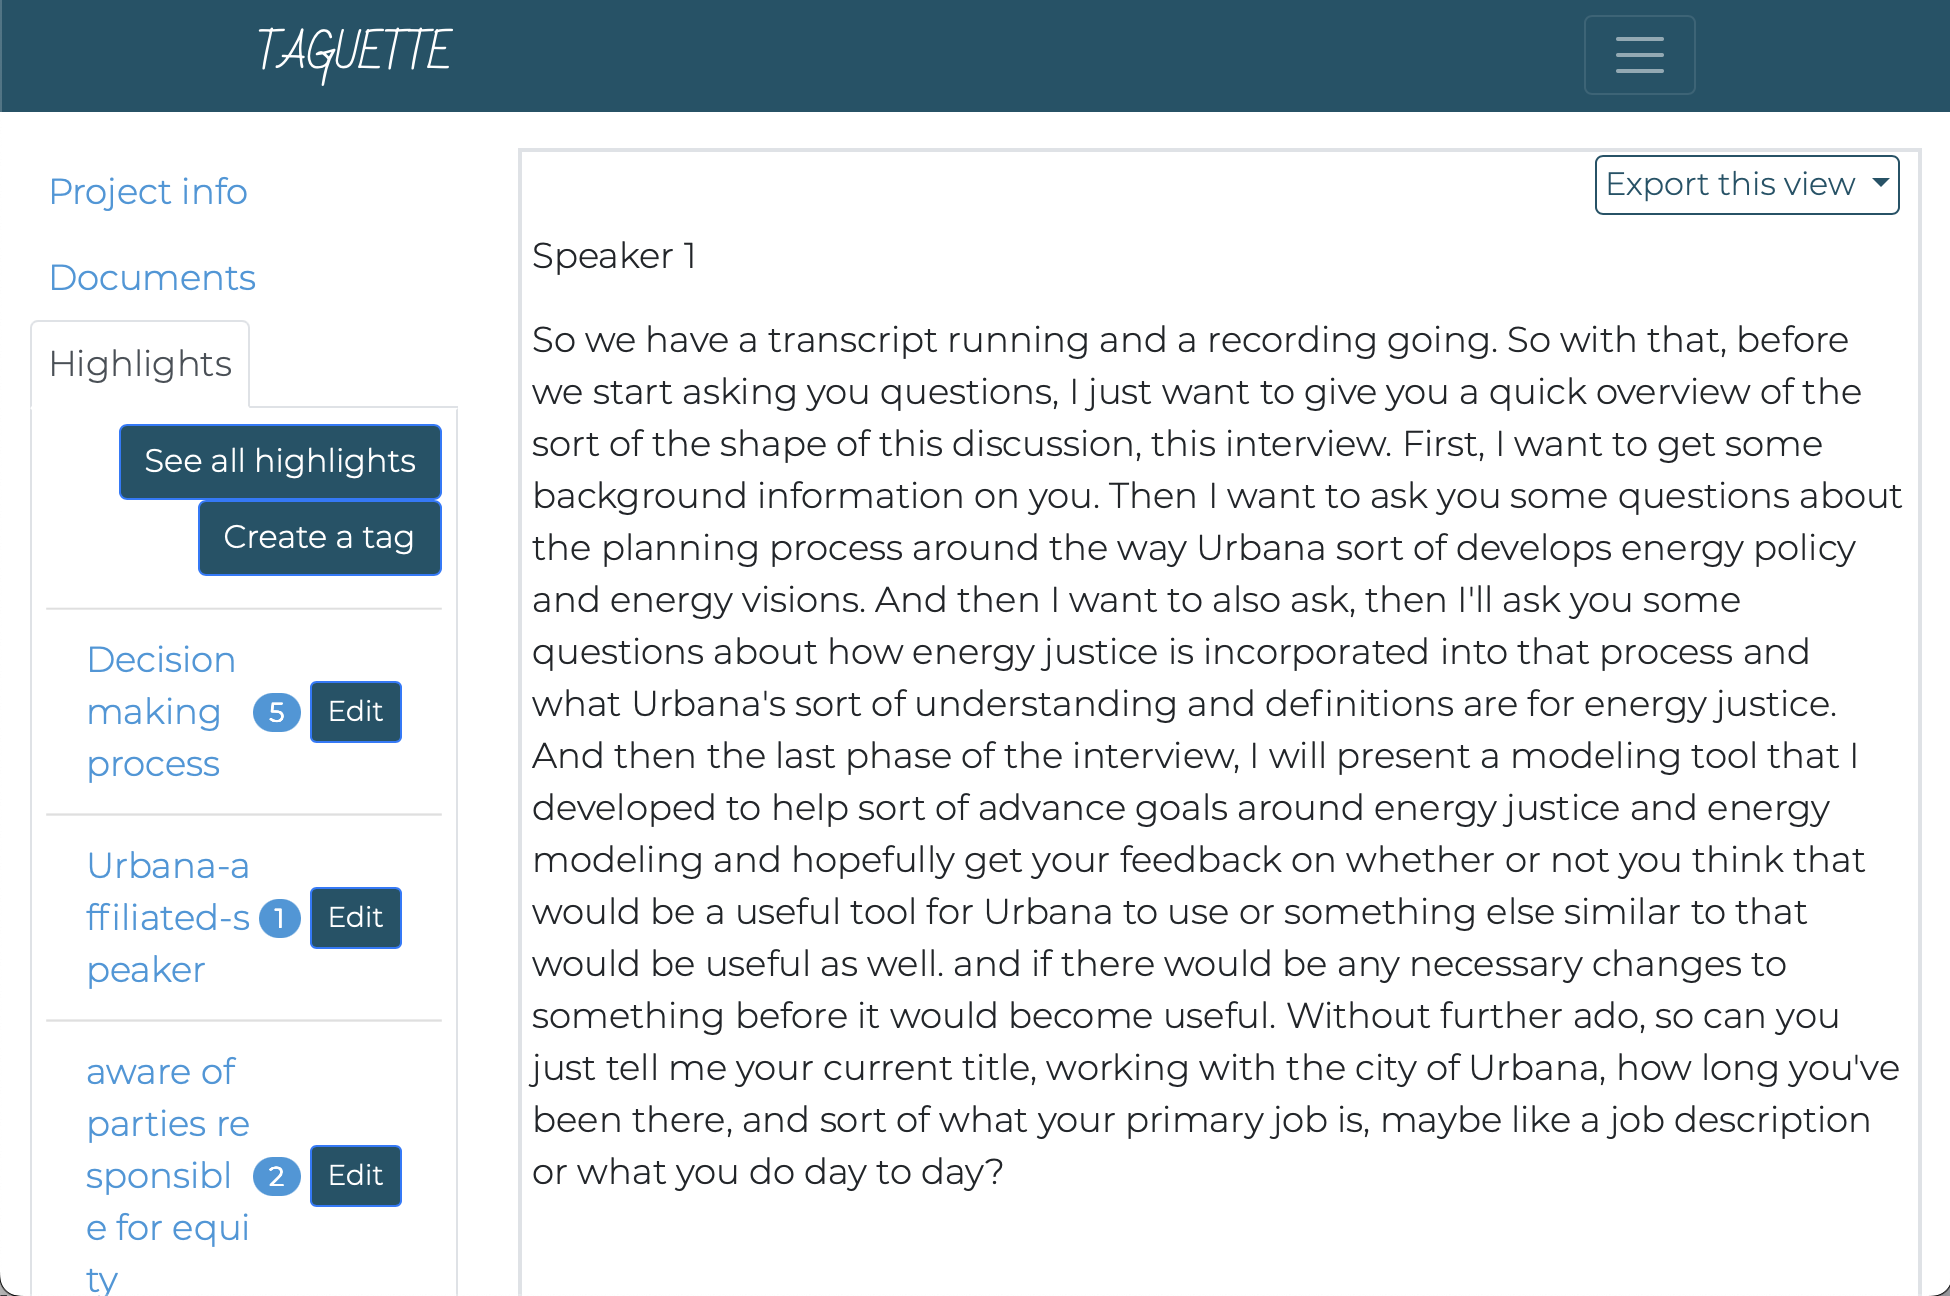
\includegraphics[width=0.6\columnwidth]{figures/07_interview_chapter/taguette-screenshot}
    \caption{A screenshot of the interview transcribed in Figure \ref{fig:whisper}
    loaded into \texttt{Taguette} for initial coding.}
    \label{fig:taguette}
\end{figure}

\subsection{Interview Data Collection}

\begin{enumerate}
    \item Who did I interview and what organizations were they from?
    \item Why did I choose these interviews?
    \item When were the interviews conducted?
    \item How were the interviews conducted? (i.e., over Zoom)
\end{enumerate}

\subsection{Case ``Municipalities''}

\textcolor{red}{These aren't all municipalities (e.g., Illinois) I'll come up with 
a better word later. This is where I want to describe the places of interest.}

\subsubsection{Champaign, Illinois}
\subsubsection{Urbana, Illinois}
\subsubsection{\acf{uiuc}}
\subsubsection{Naperville, Illinois}
Naperville is interesting because it owns the distribution utility that serves electricity
but does not own any generation.
\begin{enumerate}
    \item \ac{nest}
    \item City of Naperville (Sustainability Department)
\end{enumerate}
\subsubsection{State of Illinois}
\begin{enumerate}
    \item \ac{icc}
    \item \ac{ipa}
    \item \ac{icea}
    \item Illinois \ac{cub}
\end{enumerate}






% This chapter addresses my proposal to ``validate'' \ac{osier} by conducting a
% case study of energy planning processes in Champaign-Urbana through interviews
% with decision makers and planners about energy justice, energy modeling, and
% energy planning. As well as introduce interviewees to \ac{osier} itself and
% solicit feedback from them about its potential usefulness and what obstacles may
% interfere with its adoption. 

% Although I originally set out to conduct a limited case study of Chambana, I
% discovered that municipalities in Illinois do not, in general, have the decision
% making authority to make specific choices about their energy supply.
% Thus, I expanded my study to the state level; interviewing people from the
% \ac{ipa} and \ac{icc}. This expanded scope provided evidence for structural
% challenges blocking municipal influence from energy planning processes. Further,
% this evinces a tension among distributive, procedural, and recognition justice.

% \section{Progress on developing tools for local use}

% \begin{itemize}
%     \item The literature review chapter indicated that most energy modeling tools
%     and much of the related literature focus on state- or national-scale energy
%     systems.
%     \item The the hyper-local section highlighted some studies that integrated
%     local perspectives with energy modeling. Those papers include 
%     \cite{mckenna_combining_2018, johannsen_municipal_2023, fleischhacker_portfolio_2019}
%     \item There have also been studies investigating the development of models for, and
%     use by, city and urban planners.
% \end{itemize}

% \section{Municipal Levers: How municipalities make choices about their energy supply}
% There are generally four ways municipalities can make choices about their energy supply.

% \subsection{\ac{mca}}
% This is where municipalities participate in electricity markets on behalf of
% their residents. Although this allows municipalities to choose an energy supply
% besides the standard portfolio provided by an electric utility, municipalities
% do not have full control over their energy supply. Instead, municipalities
% negotiate for a few portfolios through a bidding process. While they can specify
% some criteria, such as a percentage of renewable energy, the specific generation
% mix depends on the company that developed the portfolio bid. Further, residents
% are still allowed to opt-out of \ac{mca} and elect the standard portfolio
% provided by their electric utility.

% \subsection{Utility ownership}
% Some municipalities in Illinois, such as Naperville, own their own distribution
% system. This gives a municipality greater control over the design of their
% utility system and allows a municipality to make decisions about the tradeoff
% between cost and resiliency. For example, Naperville undergounded most of the
% electric distribution system and new distribution is automatically undergounded.
% However, this model does not award control of electric supply to the
% municipality, which must procure electricity through another entity such as the
% \acf{imea}.

% \subsection{Municipal-owned generation}
% In very few cases, a municipality may own some of its own generation. \ac{uiuc}
% owns a coal and natural gas plant, a solar array, chilled water storage, and
% participates in a \ac{ppa} to purchase wind power. More commonly, municipalities
% will lease land cheaply to a solar company, for example, and purchase some or all
% of the rights to that electricity through a \ac{ppa}. 

% \subsection{Municipal-owned buildings}